\documentclass[a4paper,10pt]{article}
\usepackage[utf8]{inputenc}
\usepackage[T1]{fontenc}
\usepackage{textcomp}
\usepackage{eulervm}
\usepackage{amsmath}
\usepackage{amssymb}
\usepackage{amstext}
\usepackage{noweb}
\usepackage{bm}
\usepackage{hyperref}
\usepackage{color}
\usepackage{caption}
\usepackage{graphicx}

\newcommand{\argmin}[1]{\underset{#1}{\operatorname{arg}\operatorname{min}}\;}
\newcommand{\pdf}{\phi(\lambda)}
\newcommand{\pdff}{\phi(\tfrac{\lambda}{s})}
\newcommand{\pdfff}{\phi(\tfrac{\lambda'}{s})}
\newcommand{\cdf}{\Phi(\lambda)}
\newcommand{\cdff}{\Phi(\tfrac{\lambda}{s})}
\newcommand{\cdfff}{\Phi(\tfrac{\lambda'}{s})}
\newcommand{\sqb}[1]{\begin{bmatrix}#1\end{bmatrix}}
\newcommand{\C}{\mathcal{C}}
\newcommand{\N}{\mathcal{N}}
\newcommand{\inv}{^{-1}}
\newcommand{\E}{\mathbb{E}}
\newcommand{\V}{\mathbb{V}}
\definecolor{brown}{rgb}{0.54, 0.26, 0.07}
\newcommand{\brown}[1]{\textcolor{brown}{#1}} 
\newcommand{\blue}[1]{\textcolor{blue}{#1}} 

% tabbing    % http://tex.stackexchange.com/questions/73287/adding-tabs-or-creating-my-own-command
\newcommand{\itab}[1]{\hspace{0em}\rlap{#1}}
\newcommand{\tab}[1]{\hspace{.11\textwidth}\rlap{#1}}

%opening
\title{Myopic Gittins \\ Exploration Heuristic for PILCO}
\author{Rowan McAllister}

\begin{document}

\maketitle

\tableofcontents

\section{Situation}

The simulate function generates cumulative-cost \emph{distributions} $\C_\theta$ (with derivatives) for 
any controller parameterisation $\theta \in \Theta$ we input,
\begin{eqnarray}
 \C_\theta \sim \N(\mu_\theta,\sigma^2_\theta)&\;\leftarrow\;&{\tt 
simulate}(\theta)
\end{eqnarray}
Currently we do gradient decent, to select the optimal $\theta$ w.r.t. mean 
information only:
\begin{eqnarray}
 \theta^* &\;\leftarrow\;& \argmin{\theta} \sqb{\mu_\theta} 
\label{eq:currentstrategy}
\end{eqnarray}
%
In addition to cumulative-cost mean information $\mu_\theta$, we also have:
\begin{itemize}
 \item cumulative-cost uncertainty information $\sigma^2_\theta$,
 \item the number of trials left $n$. 
 %Note $n$ is different to horizon $H$ - the 
 %number of iteration in \emph{each} trial - which 
 % we assumed is fixed.
\end{itemize}
We possibly also know the equivalent `observation noise' that a sample from a rollout would give us 
(by an ability to estimate the reduction in uncertainty that would result from a future rollout).

\section{Task}

How can we find a $\theta$ that is optimal, not just w.r.t. mean information, 
but w.r.t. all:
\begin{itemize}
 \item \itab{$\mu_\theta$} \tab{mean information,}
 \item \itab{$\sigma^2_\theta$} \tab{uncertainty information,}
 \item \itab{$n$} \tab{number of trials left information.}
\end{itemize}
In addition we \textit{might} know:
\begin{itemize}
 \item \itab{$\hat{\sigma}^2_{\theta, t+1}$} \tab{estimated uncertainty of the next time iteration (default 0), or}
 \item \itab{$\sigma_y^2(\theta)$} \tab{observation noise as a function of $\theta$ (default 0 for all $\theta$).}
\end{itemize}


\section{Approximate Solution: Finite-Horizon} \label{sec:soln-optimism}

The exact solution involves infinite belief lookahead (intractable).
We therefore restrict our solution-space to myopic (one-step) lookahead solutions.
Myopic lookahead is an approximation to infinite belief lookahead,
which only considers what could plausibly be learned in the next time step,
and thereafter assumes the agent will learn nothing further.
If we can make the assumption that each Gaussian $\C_\theta$
is independent from all other $\{\C_{\theta'}:\theta' \in \Theta\neq\theta\}$,
then we apply the Gittin's index solution.

\subsection{Optimistic Approximation}
We can make the optimistic assumption that our observation noise $\sigma_y^2$ is zero.
I.e. we are about to learn everything there is to learn about our Gaussian bandit in the next time step.
With prior cumulative-cost distribution $\C^t_\theta$ , 
and applying controller parameterised by $\theta$, 
and observing the rollout data $\mathcal{D}^t$, 
the posterior cumulative-cost ($\C^{t+1}_\theta$) will collapse to a delta function:
\begin{eqnarray}
 \C^t_\theta &\;\sim\;& \N(\mu^t_\theta,\sigma^2_\theta) \\
 \mathcal{D}^t &\;\leftarrow\;& {\tt applyController}(\theta) \\
 \C^{t+1}_\theta|\mathcal{D}^t &\;\sim\;& \N(\mu^{t+1}_\theta,0)
\end{eqnarray}
This is to say, we assume that after just one rollout with parameter $\theta$, 
we will know (with certainty) the cumulative-cost of a controller parameterised by 
$\theta$. This is optimistic, since the system itself has non-negligible process 
noise and has non-negligible observations noise.

This optimism of `learning everything about $\C_\theta$ with just one 
rollout' is known in the POMDP literature as a strict upper bound on the true 
value function, usually denoted to as $V_{MDP}$ or $Q_{MDP}$. The value 
function in POMDPs is sublinear w.r.t. the belief simplex, whereas $V_{MDP}$ 
is linear (hence an upper bound). In this case we have a belief over not the 
physical state (as per usual in POMDPs), but a belief over the latent value 
function. If indeed the agent can learn everything in one rollout, then the 
upper bound is equal to the 
true value function.

\subsubsection{Computing Solution} \label{sec:computing-solution}

The solution involves:
\begin{enumerate}
 %\item using the upper bound value function $V_{MDP}(\theta)$,
 \item using a myopic look-ahead tree,
 \item computing the Gittins index (exact except for finite-horizon approximation) of our look-ahead tree (which uses number of trials $n$ information),
 \item using gradient decent w.r.t. mean \emph{and} uncertainty.
\end{enumerate}

Note we are minimising cumulative-costs here
(rather than the usual bandit setting of maximising cumulative-rewards).
OK, so we treat $\C^t_\theta$ as a bandit, and we bring in a fixed Gittins bandit which 
offers a constant cumulative-cost $\lambda$ per trial. 
For illustrative simplicity, let us initially assume our prior distribution $\C^t_\theta$ is a standard Gaussian $c \sim \N(0,1)$. The 
Gittins index is the cost of the fixed-bandit that makes us ambivalent between 
choosing the uncertain bandit and the fixed bandit, i.e.:
%
\begin{eqnarray}
  \underbrace{\C_{MDP}(\theta)}_{\text{cost of trying uncertain bandit}} 
&\;=\;& \underbrace{n\lambda}_{\text{cost of staying with fixed bandit}}
\end{eqnarray}
%
We now solve for $\lambda$. Let $\phi(\cdot)$ be the standard normal 
distribution, $\Phi(\cdot)$ its cumulative distribution function:
%
\begin{eqnarray}
 n\lambda 
 &\;=\;& \C_{MDP}(\theta) \\
 &\;=\;& \int_{-\infty}^{\infty} \phi(c)\min(\lambda,c)dc\\
 &\;=\;& \int_{-\infty}^{\lambda} \phi(c)\min(\lambda,c)dc + \int_{\lambda}^{\infty} \phi(c)\min(\lambda,c)dc\\
 &\;=\;& \int_{-\infty}^{\lambda} n\phi(c)c \, dc          + \int_{\lambda}^{\infty} \phi(c) \big( c + \lambda(n-1) \big) dc \\
 &\;=\;& (n-1)\cdot\int_{-\infty}^{\lambda} \phi(c)c \, dc          + \lambda(n-1)\cdot\int_{\lambda}^{\infty} \phi(c) dc \\
 &\;=\;& -(n-1)\pdf + \lambda(n-1)(1-\cdf) \\
 %&\;=\;& \sqb{-n\pdf} + \sqb{\pdf + (1-\cdf)\cdot\lambda (n-1)} \\
 \lambda &\;=\;& -(n-1)(\pdf+\lambda\cdf)
\end{eqnarray} 
%
%noting $\tfrac{d\pdf}{dc} = -c\cdot\pdf$.
Solve for $\lambda$ using Newton's method:
%
\begin{eqnarray}
 g_i =0 &\;=\;& (n-1)(\pdf +\lambda\cdf) + \lambda \\
 g'_i = \frac{dg_i}{d\lambda} &\;=\;& (n-1)(-\lambda\pdf +\cdf +\lambda\pdf) + 1 \\
                     &\;=\;& (n-1)\cdf + 1 \\
 \lambda_0 &\;\leftarrow\;& 0 \\
 \lambda_{i+1} &\;\leftarrow\;& \lambda_i - \frac{g_i}{g'_i}
\end{eqnarray}
%
This converges within 5-6 iterations.

\subsubsection{Using Solution}

OK great, we have this $\lambda$ value, which is a function of the number of 
trails left $n$. How do we select $\theta^*$?
%
\begin{eqnarray}
 \C_\theta \sim \N(\mu_\theta,\sigma^2_\theta)&\;\leftarrow\;&{\tt 
simulate}(\theta) \\ 
 \theta^* &\;\leftarrow\;& \argmin{\theta} \sqb{\mu_\theta - 
\lambda(n,\sigma^2_\theta)} \label{eq:newstrategy}
\end{eqnarray}
%
Note how eq~(\ref{eq:newstrategy}) equation differs with our current 
approach in PILCO, eq~(\ref{eq:currentstrategy}). Not only does 
eq~(\ref{eq:newstrategy}) utilise mean information $\mu_\theta$, as 
does eq~(\ref{eq:newstrategy}), but also uncertainty information 
$\sigma^2_\theta$, and horizon information (number of trails remaining) $n$ 
(via function $\lambda(n)$). Also note there are no free parameters!

\subsection{Pessimistic Approximation} \label{sec:soln-pessimism}

\textit{In this section we discuss the pessimistic approximation,
which is more general that the optimistic approximation
(since we can always revert to the optimistic approximation by setting observation noise to zero in this section).}

Let our current prior at time t is $\C_t \sim \N(\mu_t,\sigma^2_t)$
(dropping the inherent $\theta$ index to simplify notation).
We therefore anticipate, according to our prior, that we will receive an observation distributed as
\begin{eqnarray}
 y_t \sim \N(\C_t,\sigma_y^2)
\end{eqnarray}
%
Thus, our new posterior will be
\begin{eqnarray}
 \C_{t+1} &\;\sim\;& \N(\mu_{t+1},\sigma^2_{t+1}), \;\; \text{where} \\
 \sigma^2_{t+1} &\;=\;& (\sigma^{-2}_t + \sigma_y^{-2})\inv \label{eq:sigma-new} \\
 \mu_{t+1} &\;=\;& \sigma^2_{t+1}(\sigma^{-2}_t\mu_t + \sigma_y^{-2}y_t)
\end{eqnarray}
We now make the pessimistic assumption that the next time iteration is the only thing 
we will ever learn (according to the normal observation noise) about this particular parameterisation $\theta$. 
I.e. the mean function will be our expected reward payout from $\C_\theta$ all the way up until the horizon.

OK so what will the approximate Gittins Index look like now?
First let us note:
\begin{eqnarray}
 y_t &\;\sim\;& \N(\C_t,\sigma_y^2) \\
   &\;\sim\;& \N(\mu_t,\sigma^2_t + \sigma_y^2) \\
 \mu_{t+1} &\;=\;& \sigma^2_{t+1}(\sigma^{-2}_t\mu_t + \sigma_y^{-2}y_t) \label{eq:mu-new} \\
           &\;\sim\;& \N(\sigma^2_{t+1}(\sigma^{-2}_t\mu_t + \sigma_y^{-2}\mu_t), \;\sigma^4_{t+1}\sigma_y^{-4}(\sigma^2_t + \sigma_y^2)) \\
           % &\;\sim\;& \N(\mu_t, \;\sigma^4_{t}(\sigma^2_t + \sigma_y^2)\inv)
           % &\;\sim\;& \N(\mu_t, \;\sigma^2_{t}(1 + \tfrac{\sigma_y^2}{\sigma^2_t})\inv)
           &\;\sim\;& \N(\mu_t, \;\underbrace{\sigma^2_{t}\cdot\tfrac{\sigma^2_{t}}{(\sigma^2_t + \sigma_y^2)}}_{s^2})
\end{eqnarray}
For simple notation let $\mu = \mu_{t+1}$.
Since the Gittins index can be decomposed into a mean and additive function of variance,
then for these calculation we centre $\C_t$, i.e. $\mu_t=0$ (and will un-centre it later).
OK now the approximate pessimistic Gittins index:
\begin{eqnarray}
 n\lambda 
 &\;=\;& \int_{-\infty}^{\infty} \N(\mu;0,s^2)\min(\lambda,\mu)d\mu\\
 &\;=\;& \int_{-\infty}^{\lambda} \N(\mu;0,s^2)\min(\lambda,\mu)d\mu + \int_{\lambda}^{\infty} \N(\mu;0,s^2)\min(\lambda,\mu)d\mu\\
 &\;=\;& \int_{-\infty}^{\lambda} y+(n-1)\N(\mu;0,s^2)\mu \, d\mu + \int_{\lambda}^{\infty} \N(\mu;0,s^2) \big( y + \lambda(n-1) \big) d\mu \nonumber\\
 &\;=\;& (n-1)\cdot\int_{-\infty}^{\lambda} \N(\mu;0,s^2)\mu \, d\mu + \lambda(n-1) \cdot \int_{\lambda}^{\infty} \N(\mu;0,s^2) d\mu \nonumber\\
 &\;=\;& (n-1)\sqb{-s\pdff + \lambda(1-\cdff)} \\
 \lambda  &\;=\;& -(n-1)(s\pdff +\lambda\cdff)
\end{eqnarray} 
%
Solve for $\lambda$ using Newton's method:
%
\begin{eqnarray}
 g_i =0 &\;=\;& (n-1)(s\pdff +\lambda\cdff) + \lambda \\
 g'_i = \frac{dg_i}{d\lambda} &\;=\;& (n-1)(-\tfrac{\lambda}{s}\pdff +\cdff +\tfrac{\lambda}{s}\pdff) + 1 \\
                     &\;=\;& (n-1)\cdff + 1 \\
 \lambda_0 &\;\leftarrow\;& 0 \\
 \lambda_{i+1} &\;\leftarrow\;& \lambda_i - \frac{g_i}{g'_i}
\end{eqnarray}

\subsubsection{Example Values of $-\lambda$ for Various Inputs} 

Note $n$ is the number of trials remaining (including the current trial we are considering),
and $\sigma^2_y / \sigma_t^2$ is the ratio of the observation noise from observing a rollout and the 
prior variance.

\begin{tabular}{ c | c c c c c }
   &       \blue{$\sigma^2_y / \sigma_t^2$} &        &        &        \\
\brown{n}  &       \blue{0} &       \blue{0.1} &       \blue{1} &       \blue{10} & \blue{$\infty$} \\
\hline
\brown{1 } &      0 &      0 &      0 &      0 & 0 \\
\brown{2 } & 0.2760 & 0.2632 & 0.1952 & 0.0832 & 0 \\
\brown{3 } & 0.4363 & 0.4160 & 0.3085 & 0.1316 & 0 \\
\brown{4 } & 0.5492 & 0.5236 & 0.3883 & 0.1656 & 0 \\
\brown{5 } & 0.6360 & 0.6064 & 0.4497 & 0.1918 & 0 \\
\brown{6 } & 0.7065 & 0.6736 & 0.4996 & 0.2130 & 0 \\
\brown{7 } & 0.7658 & 0.7301 & 0.5415 & 0.2309 & 0 \\
\brown{8 } & 0.8168 & 0.7788 & 0.5776 & 0.2463 & 0 \\
\brown{9 } & 0.8616 & 0.8215 & 0.6092 & 0.2598 & 0 \\
\brown{10} & 0.9015 & 0.8595 & 0.6374 & 0.2718 & 0 \\
\end{tabular}

% \section{Approximate Solution C: \\ \large{Optimistic and Infinite-Horizon}}
% 
% Similar to solution I (Sec.\ref{sec:soln-optimism}), but with infinite horizon and discounting $\gamma$.
% Note the value of getting reward $\lambda$ from now until forever more is $\frac{\lambda}{1-\gamma}$.
% 
% \begin{eqnarray}
%  \frac{\lambda}{1-\gamma} 
%  &\;=\;& \int_{-\infty}^{\lambda} \phi(z)V^*(z)dz + \int_{\lambda}^{\infty} \phi(z)V^*(z)dz\\
%  &\;=\;& \int_{-\infty}^{\lambda} \phi(z) \big( z + \frac{\lambda\gamma}{1-\gamma} \big) dz + \int_{\lambda}^{\infty} \phi(z)\frac{z}{1-\gamma} \, dz \\
%  &\;=\;& -\pdf + \cdf\cdot\frac{\lambda\gamma}{1-\gamma} + \frac{\pdf}{1-\gamma} \\
%  % &\;=\;& \cdf\cdot\frac{\lambda\gamma}{1-\gamma} + \frac{\pdf\gamma}{1-\gamma} \\
%  &\;=\;& \frac{\gamma}{1-\gamma}\cdot(\pdf +\lambda\cdf)
% \end{eqnarray} 
% %
% Solve for $\lambda$ using Newton's method:
% %
% \begin{eqnarray}
%  g_i =0 &\;=\;& \gamma\cdot(\pdf +\lambda\cdf) - \lambda \\
%  g'_i = \frac{dg_i}{d\lambda} &\;=\;& \gamma\cdot(-\lambda\pdf +\cdf +\lambda\pdf) - 1 \\
%                      &\;=\;& \gamma\cdot\cdf - 1 \\
%  \lambda_0 &\;\leftarrow\;& 0 \\
%  \lambda_{i+1} &\;\leftarrow\;& \lambda_i - \frac{g_i}{g'_i}
% \end{eqnarray}

\subsubsection{Derivatives} \label{sec:derivatives-finite}

How would $\lambda$ change for small changes in $\sigma_t^2$?
To answer this, we first define $\lambda$ as a function of $s$, i.e. $\lambda(s)$
(noting that $s$ is the only variable that is directly a function of $\sigma_t^2$),
and determine how $\lambda$ would respond to changes in $s$ such that the constraint $g=0$
is still satisfied.
I.e.:
\begin{eqnarray}
 g =  0 &\;=\;& (n-1)(s\pdff +\lambda\cdff) + \lambda \\
 \therefore \frac{dg}{ds} = 0 &\;=\;& (n-1)(\pdff +\frac{d\lambda}{ds}\cdff) + \frac{d\lambda}{ds} \\
 \therefore \frac{d\lambda}{ds} &\;=\;& -\frac{\pdff}{\cdff+1/(n-1)}
\end{eqnarray}
Now note:
\begin{eqnarray}
 \frac{d\lambda}{d\sigma_t^2} &\;=\;& \frac{d\lambda}{ds} \cdot \frac{ds}{d\sigma_t^2} \\
  &\;=\;& \frac{d\lambda}{ds} \cdot \Big[ \frac{ \sqrt{\sigma_t^2+\sigma_y^2} - s/2}{\sigma_t^2+\sigma_y^2}\Big]
\end{eqnarray}

%\newpage
%\section{Approximate Solution D: \\ \large{Pessimistic and Infinite-Horizon}}
\section{Approximate Solution: Infinite-Horizon}

Similar to solution in Sec.~\ref{sec:soln-pessimism}, but with infinite horizon and discounting $\gamma$.

\begin{eqnarray}
 \frac{\lambda}{1-\gamma}
 &\;=\;& \int_{-\infty}^{\lambda} \N(\mu;0,s^2)\min(\lambda,\mu)d\mu + \int_{\lambda}^{\infty} \N(\mu;0,s^2)\min(\lambda,\mu)d\mu\\
 &\;=\;& \int_{-\infty}^{\lambda} y+\N(\mu;0,s^2)\frac{\mu\gamma}{1-\gamma} \, d\mu + \int_{\lambda}^{\infty} \N(\mu;0,s^2) \big( y + \frac{\lambda\gamma}{1-\gamma} \big) d\mu \nonumber\\
 &\;=\;& -\frac{s\gamma}{1-\gamma}\cdot\pdff + \frac{\lambda\gamma}{1-\gamma}\cdot(1-\cdff)  \\
 \lambda &\;=\;& -\frac{\gamma}{1-\gamma}\cdot(s\pdff +\lambda\cdff)
\end{eqnarray} 
%
Solve for $\lambda$ using Newton's method:
%
\begin{eqnarray}
 g_i =0 &\;=\;& \gamma\cdot(s\pdff +\lambda\cdff) + \lambda(1-\gamma) \\
        &\;=\;& \gamma\cdot(s\pdff +\lambda\cdff-\lambda) + \lambda \\
 g'_i = \frac{dg_i}{d\lambda} &\;=\;& \gamma\cdot(-\tfrac{\lambda}{s}\pdff +\cdff +\tfrac{\lambda}{s}\pdff-1) + 1 \\
                     &\;=\;& \gamma\cdot(\cdff-1)+1\\
 \lambda_0 &\;\leftarrow\;& 0 \\
 \lambda_{i+1} &\;\leftarrow\;& \lambda_i - \frac{g_i}{g'_i}
\end{eqnarray}

\subsection{Derivatives}

Similar to Sec.~\ref{sec:derivatives-finite}, we have:

\begin{eqnarray}
 g =  0 &\;=\;& \gamma\cdot(s\pdff +\lambda\cdff) + \lambda(1-\gamma) \\
 \therefore \frac{dg}{ds} = 0 &\;=\;& \gamma\cdot(\pdff +\frac{d\lambda}{ds}\cdff) + \frac{d\lambda}{ds}(1-\gamma) \\
 \therefore \frac{d\lambda}{ds} &\;=\;& -\frac{\pdff}{\cdff-1 + 1/\gamma}
\end{eqnarray}
Now note:
\begin{eqnarray}
 \frac{d\lambda}{d\sigma_t^2} &\;=\;& \frac{d\lambda}{ds} \cdot \frac{ds}{d\sigma_t^2} \\
  &\;=\;& \frac{d\lambda}{ds} \cdot \Big[ \frac{ \sqrt{\sigma_t^2+\sigma_y^2} - s/2}{\sigma_t^2+\sigma_y^2}\Big]
\end{eqnarray}

\subsection{Bounds} 

\begin{figure}[h]
\centering
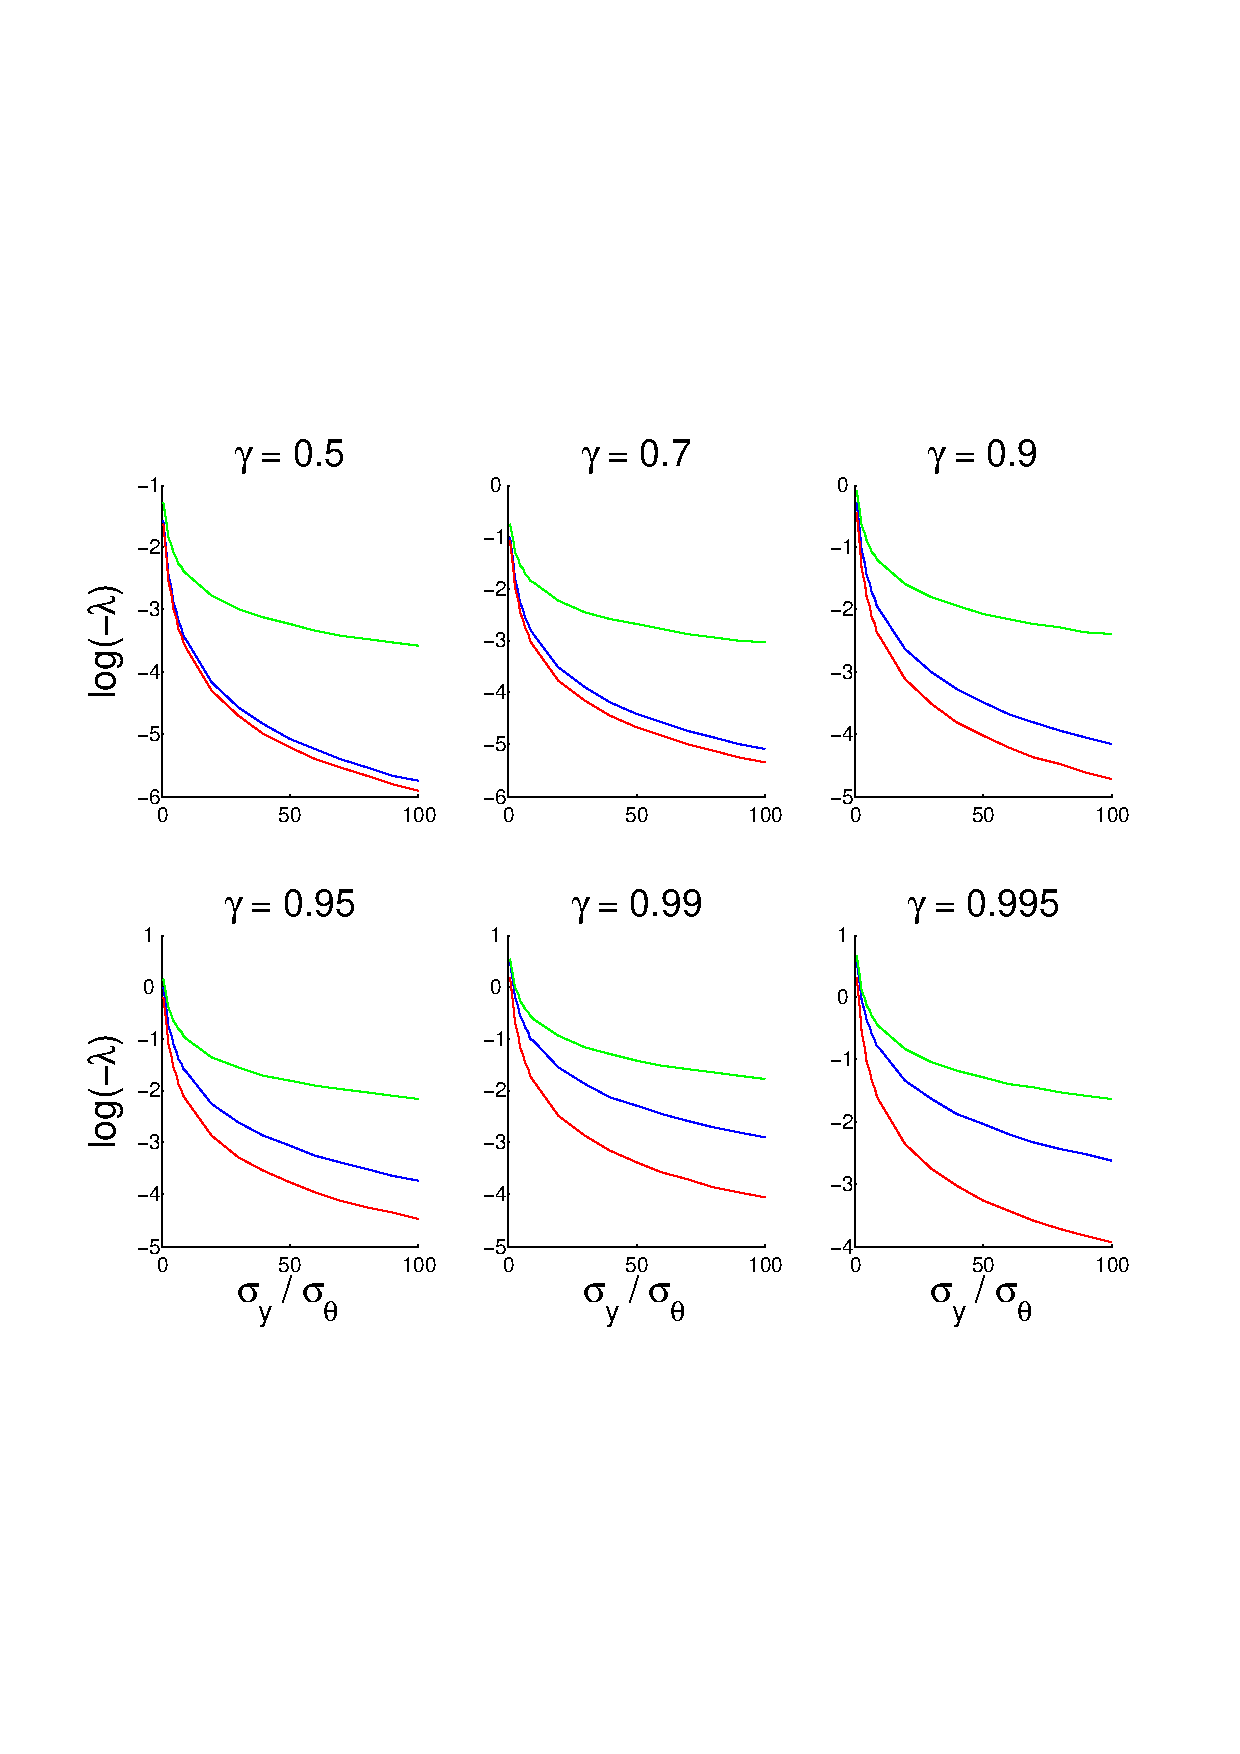
\includegraphics[width=0.81\linewidth]{bounds.pdf}
\caption{Bounds: The blue line is the exact Gittins index for infinite horizon.
The Gittins index is upper bounded by the green line - which is the optimistic approximation to infinite horizon case.
The Gittins index is also lower bounded by the red line - which is the pessimistic approximation to infinite horizon case.
We set $\sigma_y=1$.}
\end{figure}

\end{document}
